\documentclass{article}
\usepackage[utf8]{inputenc}
\usepackage{graphicx}

\title{LabMuoni}
\author{giulia lavizzari}
\date{November 2021}

\begin{document}

\maketitle

\section{12/11/21}
Primo approcio alla strumentazione. Sembrava ancora che le cose funzionassero :)

\section{17/11/21}
Caratterizzazione dei moduli
\\\\\textbf{Discriminator threshold settings:}
\begin{itemize}
    \item range threshold
    \item corrispondenza tra valore della soglia e altezza dell'impulso
\end{itemize}\
\textbf{Timer counter settings:}
\begin{itemize}
    \item lo stesso numero di conteggi viene osservato con tutti i canali (impulsatore $\rightarrow$ discriminatore con soglia bassa $\rightarrow$ counter)
\end{itemize}


\section{19/11/21}
\textbf{Caratterizzazione dei moduli con impulsatore (onde quadre) e caratterizzazione risposta scintillatore con scelta della soglia}\\\\
Carattatterizzazione nuovo discriminatore: range soglia per ogni canale, risposta corretta del modulo all'onda quadra.\\\\
Scelta della soglia: discriminatore + scintillatore zero. Plot rate vs thr, si cerca il plateau. HV = 900V, t=100s
\begin{figure}
    \centering
    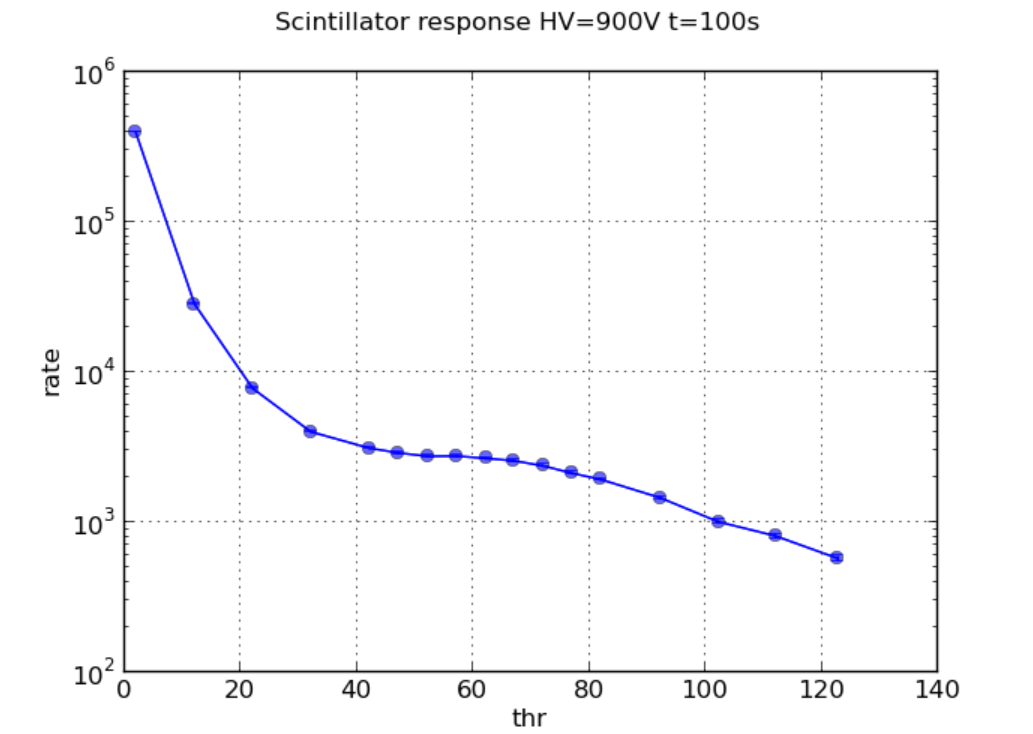
\includegraphics[width=0.9\textwidth]{plot1.png}
\end{figure}
\end{document}
